%%%%%%%%%%%%%%%%%%%%%%%%%%%%%%%%%%%%%%%%%
% Beamer Presentation
% LaTeX Template
% Version 1.0 (10/11/12)
%
% This template has been downloaded from:
% http://www.LaTeXTemplates.com
%
% License:
% CC BY-NC-SA 3.0 (http://creativecommons.org/licenses/by-nc-sa/3.0/)
%
%%%%%%%%%%%%%%%%%%%%%%%%%%%%%%%%%%%%%%%%%

%----------------------------------------------------------------------------------------
%	PACKAGES AND THEMES
%----------------------------------------------------------------------------------------

\documentclass{beamer}

\mode<presentation> {

% The Beamer class comes with a number of default slide themes
% which change the colors and layouts of slides. Below this is a list
% of all the themes, uncomment each in turn to see what they look like.

%\usetheme{default}
%\usetheme{AnnArbor}
%\usetheme{Antibes}
%\usetheme{Bergen}
%\usetheme{Berkeley}
%\usetheme{Berlin}
%\usetheme{Boadilla}
\usetheme{CambridgeUS}
%\usetheme{Copenhagen}
%\usetheme{Darmstadt}
%\usetheme{Dresden}
%\usetheme{Frankfurt}
%\usetheme{Goettingen}
%\usetheme{Hannover}
%\usetheme{Ilmenau}
%\usetheme{JuanLesPins}
%\usetheme{Luebeck}
%\usetheme{Madrid}
%\usetheme{Malmoe}
%\usetheme{Marburg}
%\usetheme{Montpellier}
%\usetheme{PaloAlto}
%\usetheme{Pittsburgh}
%\usetheme{Rochester}
%\usetheme{Singapore}
%\usetheme{Szeged}
%\usetheme{Warsaw}

% As well as themes, the Beamer class has a number of color themes
% for any slide theme. Uncomment each of these in turn to see how it
% changes the colors of your current slide theme.

%\usecolortheme{albatross}
%\usecolortheme{beaver}
%\usecolortheme{beetle}
%\usecolortheme{crane}
%\usecolortheme{dolphin}
%\usecolortheme{dove}
%\usecolortheme{fly}
%\usecolortheme{lily}
%\usecolortheme{orchid}
%\usecolortheme{rose}
%\usecolortheme{seagull}
%\usecolortheme{seahorse}
%\usecolortheme{whale}
%\usecolortheme{wolverine}

%\setbeamertemplate{footline} % To remove the footer line in all slides uncomment this line
%\setbeamertemplate{footline}[page number] % To replace the footer line in all slides with a simple slide count uncomment this line

%\setbeamertemplate{navigation symbols}{} % To remove the navigation symbols from the bottom of all slides uncomment this line
}

\usepackage{graphicx} % Allows including images
\usepackage{booktabs} % Allows the use of \toprule, \midrule and \bottomrule in tables
\usepackage{dsfont}
\usepackage{subfig}
%----------------------------------------------------------------------------------------
%	TITLE PAGE
%----------------------------------------------------------------------------------------

\title[Logistic Regression]{Logistic Regression} % The short title appears at the bottom of every slide, the full title is only on the title page

\author{Wenzhen Zhu, Sayantan Bhadra, Cancan Li, Charlie Wu, Chih Yun Pai} % Your name
\institute[WUSTL] % Your institution as it will appear on the bottom of every slide, may be shorthand to save space
{
Washington University in St. Louis \\ % Your institution for the title page
\medskip
\textit{@wustl.edu} % Your email address
}
\date{\today} % Date, can be changed to a custom date

\begin{document}

\begin{frame}
\titlepage % Print the title page as the first slide
\end{frame}

%----------------------------------------------------------------------------------------
%	PRESENTATION SLIDES Section 2
%----------------------------------------------------------------------------------------

\begin{frame}
\frametitle{Logistic Regression}
\begin{itemize}
\item Binary Classification
\item Multi-class Classification
\end{itemize}
\end{frame}

%------------------------------------------------
\begin{frame}
\frametitle{Fisher's Iris}
The data set consists of 50 samples from each of three 
species of iris flowers.  Four features were measured from each
sample, they are the length and the width of sepal and petal. This data set is often used
to demonstrate classification techniques and discriminant analysis.
\begin{figure}[htbp] \centering \subfloat[setosa]{
    \label{fig:subfig_a}
    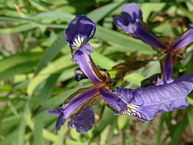
\includegraphics[scale=.4]{graphics/setosa}
}
\hspace{20pt} \subfloat[versicolor]{
    \label{fig:subfig_b}
    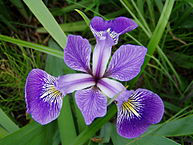
\includegraphics[scale=.4]{graphics/versicolor}
}
\hspace{20pt} \subfloat[virginica]{
    \label{fig:subfig_c}
    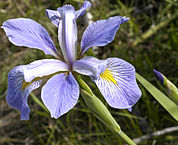
\includegraphics[scale=.4]{graphics/virginica}
}
\caption{Iris } \end{figure}
\end{frame}

%------------------------------------------------
\begin{frame}
\frametitle{Fisher's Iris}
Four features were measured from each
sample, they are the length and the width of sepal and petal.
\begin{figure}[htbp]
\centering
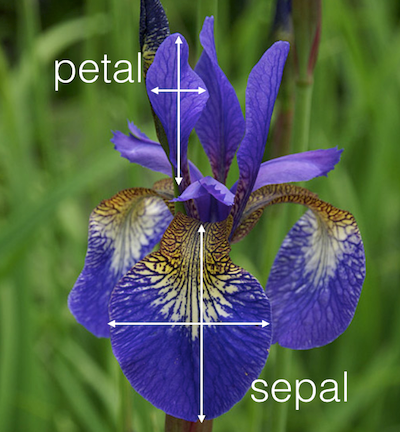
\includegraphics[scale=.35]{graphics/iris_feature} \caption{Features}
\label{fig:Features}
\end{figure}
\end{frame}
%------------------------------------------------
\begin{frame}
\frametitle{Sample Data}
\begin{table}
\begin{tabular}{lllll}
\hline
\textbf{Sepal Length} & \textbf{ Sepal Width } & \textbf{Petal Length} & \textbf{Petal Width} & \textbf{Species}\\
\hline
5.8 & 4.   & 1.2 & 0.2 & setosa\\
6.4 & 2.8 & 5.6 & 2.1 & virginica\\
6.7 & 3.1 & 5.6 & 2.4 & virginica \\
\hline
\end{tabular}
\caption{Fisher's Iris Dataset Sample}
\end{table}
\end{frame}
%------------------------------------------------
\begin{frame}
\frametitle{Visualization of Iris Dataset}
\begin{figure}[t]
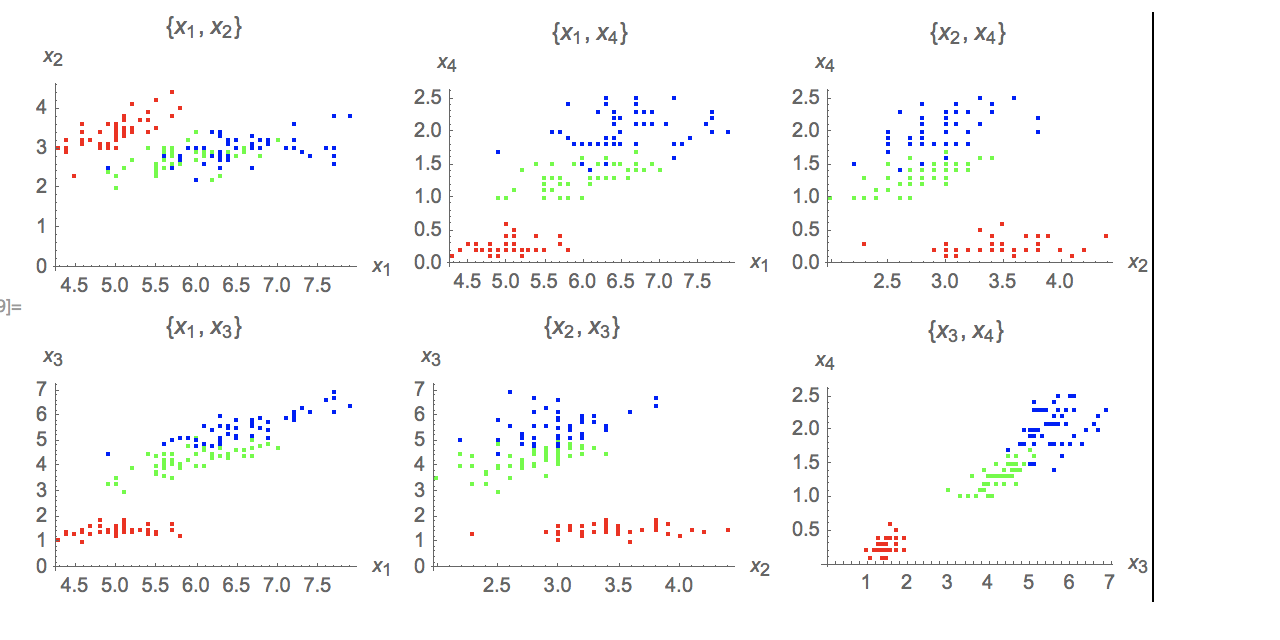
\includegraphics[scale=0.5]{graphics/feature_vis}
\centering
\end{figure}
\end{frame}
%------------------------------------------------

\begin{frame}
\frametitle{}
\[\text{Let's start from binary classification y $\in $ $\{$0, 1$\}$}\]

\[\text{y $\in $ $\{$0, 1$\}$   0 $\to $ versicolor 1$\to $ virginica}\]
\[	
	x = (x_ 1, x_ 2) \
		where \ x_1 = \text{sepal width}, x_2 = \text{petal width}\]
\end{frame}

%------------------------------------------------
\begin{frame}
\frametitle{Sigmoid Function 1D}
\[h(x)=\frac{1}{1+e^{-x}}\]
\begin{figure}[t]
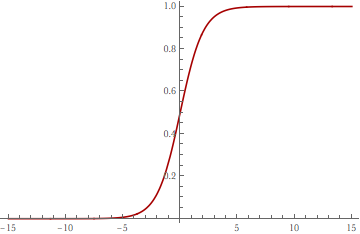
\includegraphics[width=5cm]{graphics/1d-sigmoid}
\centering
\end{figure}
\end{frame}

%------------------------------------------------
\begin{frame}
\begin{figure}[t]
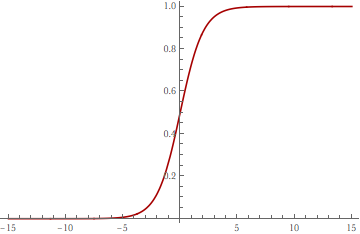
\includegraphics[width=5cm]{graphics/1d-sigmoid}
\centering
\end{figure}
\[h(x)>=\frac{1}{2}  \Rightarrow class 1\]
\[h(x)<\frac{1}{2}  \Rightarrow class 0\]
\[h(x)=P(y=1|x)\]
\[1-h(x)=P(y=0|x)\]
\end{frame}
%------------------------------------------------
\begin{frame}
3D Visualization \\
See a Mathematica Dynamic Visualization
\end{frame}
%------------------------------------------------
\begin{frame}
\frametitle{Maximum Likelihood}
\begin{equation}
L = \prod_{i=1}^n P(y = y^{(i)}  | x = x^{(i)}) 
= \prod_{y^{(i)} = 0 } (1-h(x^{(i)})) \prod_{y^{(i)} = 1 } (h(x^{(i)}))
\end{equation}
\begin{equation}
l =  \log (L) = \sum_{y^{(i)} = 0 } \log (1-h(x^{(i)})) \sum_{y^{(i)} = 1} \log (h(x^{(i)}))
\end{equation}
\end{frame}

%----------------------------------------------------------------------------------------
%	PRESENTATION SLIDES Section 1
%----------------------------------------------------------------------------------------
\begin{frame}
\frametitle{Binary classification} % Table of contents slide, comment this block out to remove it
\tableofcontents % Throughout your presentation, if you choose to use \section{} and \subsection{} commands, these will automatically be printed on this slide as an overview of your presentation
\section{Key problem in supervised machine learning.}
%------------------------------------------------
\section{Predict binary output from input variables, e.g.}
%Examples:
%\begin{itemize}
\subsection{Spam or not spam}
\subsection{Disease or no disease}
\subsection{Rain or no rain}
\subsection{Win or lose election etc.}
%\end{itemize}
%\section{Binary classification} % Sections can be created in order to organize your presentation into discrete blocks, all sections and subsections are automatically printed in the table of contents as an overview of the talk
%------------------------------------------------

%\subsection{Spam or not spam} % A subsection can be created just before a set of slides with a common theme to further break down your presentation into chunks
%\subsection{Disease or no disease etc.}
\section{Simplest classifiers: linear classifiers.}
\end{frame}

\begin{frame}
\frametitle{Linear classification}
Output binary class (0 or 1) based on where a linear combination of the input feature vector lies with respect to the decision boundary:
\begin{equation}
y = \frac{1}{2}(1 + \text{sign} (\theta^T x))
\end{equation}
$x \in \mathds{R}^{n+1}, \theta \in \mathds{R}^{n+1}; y \in \{0,1\}.$\\

\begin{itemize}
\item $ \theta^T x = 0 \implies \text{decision boundary}$
\item $ \theta^T x > 0 \implies y = 1$
\item $ \theta^T x  < 0 \implies y = 0$
\end{itemize}


The decision boundary (i.e. $\theta$) is learned from the training data.
\end{frame}

\begin{frame}
\frametitle{Linear classification (contd.)}
%\begin{figure}
%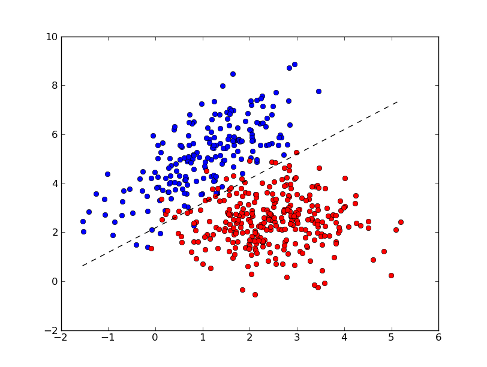
\includegraphics[width=0.6\linewidth]{lda_binary.png}
%\caption{Example of linear classification}
%\end{figure}
\end{frame}

\begin{frame}
\frametitle{Hard vs. soft threshold}
\begin{itemize}
\item Exact binary prediction (\textit{hard threshold}) may be impractical - does not reveal the confidence in the prediction.
\item Express as \textit{probability} of belonging to a class (\textit{soft threshold}), e.g. probability of raining, probability of a heart disease etc. \item Instead of a strict binary value, the classifier output is a real number between 0 and 1 - interpreted as class probability.
\item This leads to \textbf{logistic regression}.
\end{itemize}
\end{frame}

\begin{frame}
\frametitle{Modeling conditional probabilities}
\begin{itemize}
\item Determine a conditional probability distribution, or \textit{likelihood} $Pr(Y|X)$ that best describes the observed data.
\item Assuming $Pr(Y=1|X=x) = p(x;\theta)$ for some function $p$ parameterized by $\theta$ and with $i.i.d.$ observation variables, the conditional likelihood function $P(Y|X)$ is,
\begin{equation}
\prod_{i=1}^n Pr(Y=y_i|X=x_i) = \prod_{i=1}^n p(x_i;\theta)^{y_i} (1-p(x_i;\theta)^{1-y_i})
\end{equation}
\item Estimate $\theta$ by \textit{maximum likelihood estimation}.  
\end{itemize}
\end{frame}

\begin{frame}
\frametitle{Paragraphs of Text}
Sed iaculis dapibus gravida. Morbi sed tortor erat, nec interdum arcu. Sed id lorem lectus. Quisque viverra augue id sem ornare non aliquam nibh tristique. Aenean in ligula nisl. Nulla sed tellus ipsum. Donec vestibulum ligula non lorem vulputate fermentum accumsan neque mollis.\\~\\

Sed diam enim, sagittis nec condimentum sit amet, ullamcorper sit amet libero. Aliquam vel dui orci, a porta odio. Nullam id suscipit ipsum. Aenean lobortis commodo sem, ut commodo leo gravida vitae. Pellentesque vehicula ante iaculis arcu pretium rutrum eget sit amet purus. Integer ornare nulla quis neque ultrices lobortis. Vestibulum ultrices tincidunt libero, quis commodo erat ullamcorper id.
\end{frame}

%------------------------------------------------

\begin{frame}
\frametitle{Bullet Points}
\begin{itemize}
\item Lorem ipsum dolor sit amet, consectetur adipiscing elit
\item Aliquam blandit faucibus nisi, sit amet dapibus enim tempus eu
\item Nulla commodo, erat quis gravida posuere, elit lacus lobortis est, quis porttitor odio mauris at libero
\item Nam cursus est eget velit posuere pellentesque
\item Vestibulum faucibus velit a augue condimentum quis convallis nulla gravida
\end{itemize}
\end{frame}

%------------------------------------------------

\begin{frame}
\frametitle{Blocks of Highlighted Text}
\begin{block}{Block 1}
Lorem ipsum dolor sit amet, consectetur adipiscing elit. Integer lectus nisl, ultricies in feugiat rutrum, porttitor sit amet augue. Aliquam ut tortor mauris. Sed volutpat ante purus, quis accumsan dolor.
\end{block}

\begin{block}{Block 2}
Pellentesque sed tellus purus. Class aptent taciti sociosqu ad litora torquent per conubia nostra, per inceptos himenaeos. Vestibulum quis magna at risus dictum tempor eu vitae velit.
\end{block}

\begin{block}{Block 3}
Suspendisse tincidunt sagittis gravida. Curabitur condimentum, enim sed venenatis rutrum, ipsum neque consectetur orci, sed blandit justo nisi ac lacus.
\end{block}
\end{frame}

%------------------------------------------------

\begin{frame}
\frametitle{Multiple Columns}
\begin{columns}[c] % The "c" option specifies centered vertical alignment while the "t" option is used for top vertical alignment

\column{.45\textwidth} % Left column and width
\textbf{Heading}
\begin{enumerate}
\item Statement
\item Explanation
\item Example
\end{enumerate}

\column{.5\textwidth} % Right column and width
Lorem ipsum dolor sit amet, consectetur adipiscing elit. Integer lectus nisl, ultricies in feugiat rutrum, porttitor sit amet augue. Aliquam ut tortor mauris. Sed volutpat ante purus, quis accumsan dolor.

\end{columns}
\end{frame}

%------------------------------------------------

%------------------------------------------------

\begin{frame}
\frametitle{Table}
\begin{table}
\begin{tabular}{l l l}
\toprule
\textbf{Treatments} & \textbf{Response 1} & \textbf{Response 2}\\
\midrule
Treatment 1 & 0.0003262 & 0.562 \\
Treatment 2 & 0.0015681 & 0.910 \\
Treatment 3 & 0.0009271 & 0.296 \\
\bottomrule
\end{tabular}
\caption{Table caption}
\end{table}
\end{frame}

%------------------------------------------------

\begin{frame}
\frametitle{Theorem}
\begin{theorem}[Mass--energy equivalence]
$E = mc^2$
\end{theorem}
\end{frame}

%------------------------------------------------

\begin{frame}[fragile] % Need to use the fragile option when verbatim is used in the slide
\frametitle{Verbatim}
\begin{example}[Theorem Slide Code]
\begin{verbatim}
\begin{frame}
\frametitle{Theorem}
\begin{theorem}[Mass--energy equivalence]
$E = mc^2$
\end{theorem}
\end{frame}\end{verbatim}
\end{example}
\end{frame}

%------------------------------------------------

\begin{frame}
\frametitle{Figure}
Uncomment the code on this slide to include your own image from the same directory as the template .TeX file.
%\begin{figure}
%\includegraphics[width=0.8\linewidth]{test}
%\end{figure}
\end{frame}

%------------------------------------------------

\begin{frame}[fragile] % Need to use the fragile option when verbatim is used in the slide
\frametitle{Citation}
An example of the \verb|\cite| command to cite within the presentation:\\~

This statement requires citation \cite{p1}.
\end{frame}

%------------------------------------------------

\begin{frame}
\frametitle{References}
\footnotesize{
\begin{thebibliography}{99} % Beamer does not support BibTeX so references must be inserted manually as below
\bibitem[Smith, 2012]{p1} John Smith (2012)
\newblock Title of the publication
\newblock \emph{Journal Name} 12(3), 45 -- 678.
\end{thebibliography}
}
\end{frame}

%------------------------------------------------

\begin{frame}
\Huge{\centerline{The End}}
\end{frame}

%----------------------------------------------------------------------------------------

\end{document} 